\documentclass[T,J]{fose}
\taikai{2024}

\usepackage [dvipdfmx] {graphicx} 
\usepackage{ascmac}
\usepackage{url}
\usepackage{multicol}

\begin{document}

\title{マイクロサービスにおける\\コードクローンの言語間分析}
\setetitle{Cross-Language Analysis of Code Clones in Microservices}

\author{太田 悠希 吉田 則裕 崔 恩瀞 槇原 絵里奈 横井 一輝
\ejtitle{\etitle}
\shozoku{Yuki Ota, Norihiro Yoshida, Erina Makihara}{立命館大学}{Ritsumeikan University}
\shozoku{Eunjong Choi}{京都工芸繊維大学}{Kyoto Institute of Technology}
\shozoku{Kazuki Yokoi}{株式会社NTTデータグループ}{NTT DATA Group Corporation}
}

\Jabstract{
マイクロサービスとは,複雑なソフトウェアを相互に通信可能な小規模サービス群に分割するアーキテクチャスタイルである.
既存研究おいて,マイクロサービスの各サービスは小規模なプログラムで実現されているにもかかわらず,多くのサービスにコードクローンが含まれていることが報告されている.
また,それらコードクローンの同時修正が報告されており,マイクロサービスにおいてコードクローンが保守コストを増大させていることがわかっている.
しかし,既存研究が行った調査では,8個のみのプロジェクトに含まれるサービスを対象としており,それらサービスはすべてJavaで開発されている.
そのため,様々な言語で開発された多くのサービスを対象とした調査を行うと,Moらの調査とは大きく異なる結果が得られる可能性がある.
そこで本研究では,12言語で開発された284個のプロジェクトを対象としてマイクロサービスに含まれるコードクローンの調査を行った.
その結果,C\#はプログラム全体におけるコードクローンの割合や,複数のコードクローンが同時に修正されるものの割合が高いことがわかった.}
\Eabstract{}

\maketitle \thispagestyle {empty}

\section{はじめに}

マイクロサービスとは,複雑なソフトウェアを相互に通信可能な小規模サービス群に分割するアーキテクチャスタイルである\cite{Honda2023,mo2021existence,zhao2022}.
マイクロサービスの特徴の1つは,疎結合なサービス群に分割することで,各サービスの開発やデプロイ,保守を独立して行うことができることである\cite{mo2021existence,zhao2022}.

マイクロサービスを採用したプロジェクトにおいて,モジュール性を考慮しながら小規模サービス群に分割されているのであれば,各サービスに含まれるコードクローンは少ないことが予想される.
%しかし,Moらの研究では,対象としたサービスの多くにコードクローンが含まれていることが報告されている\cite{mo2021existence}.
しかし,Moらの研究では,対象としたサービスの多くにコードクローンが含まれていると報告されている\cite{mo2021existence}.
また,それらコードクローンの同時修正が報告されており,マイクロサービスにおいてコードクローンが保守コストを増大させていることがわかっている\cite{mo2021existence}.
これらMoら研究成果は,マイクロサービスを採用したプロジェクトに対して,コードクローンのライブラリ化を支援するなどの保守支援が必要であることを示唆している.
マイクロサービスでは,各サービスを独立して開発できるため,各サービスはJavaだけでなく様々な言語で開発されているにもかかわらず,Moらの調査対象はJavaで開発されたサービスのみである.
そのため,他言語で開発されたプロジェクトがマイクロサービスを採用していたときに,コードクローンに対して保守支援が必要かどうかはわかっていない.
%そのため,マイクロサービスに含まれるコードクローンについて,大規模な調査を行い,
%マイクロサービスでは,各サービスを独立して開発できるため,各サービスはJavaだけでなく様々な言語で開発されている(表\ref{table:detectLanguages}参照).
%そのため,対象言語を拡大した

そこで本研究では,マイクロサービスにおけるコードクローンに関して,対象を12言語に拡大し,保守支援の必要性を調査した.
具体的には,d'Aragonaらが収集したマイクロサービスの大規模データセット\cite{amoroso2024dataset}を対象として,クローン率や同時修正率に関して言語間分析を行った.
本稿において,クローン率はプログラム全体に対するコードクローンの割合を指し,同時修正率は全クローンセット(\ref{subsec:clone}節参照)のうちの同時修正されるものの割合を指す.
分析対象の284個のOSSプロジェクトは,Javaを含む12言語\footnote{CとC++は,1つの言語として数えている.この理由は,本研究で使用したコードクローン検出ツールであるCCFinderSWが,これらを1つの言語として扱うからである.}で記述されている.

本分析では,以下の3つのRQを設定した.
\begin{description}
    \item[RQ1:] クローン率が高い言語はどれか?
    \item[RQ2:] プロダクトコードとテストコード間でクローン率に差異はあるか?
    \item[RQ3:] コードクローンに対する同時修正率が高い言語はどれか?
\end{description}
RQ1とRQ3では,各言語で記述されたコードクローンに対して保守支援の必要性を調査するために,各言語のクローン率や同時修正率を計測した.
RQ2では,言語ごとにテストフレームワークが異なることから,テストコードのクローン率や同時修正率が言語間で異なると考え,プロダクトコードとテストコードを分けて計測を行った.
%これらのことから,以下の3つのRQを設定した.

12言語で記述されたプログラムに対してコードクローン検出を行うため,容易に対応言語を増やすことが可能な検出ツールであるCCFinderSW\cite{CCFinderSW}を用いた.CCFinderSWは,CCFinder\cite{CCFinder}と同じくトークン列の等価性に基づくType-2クローン(\ref{subsec:clone}節参照)を検出する.
分析結果の概要を以下に示す.
\begin{itemize}
    \item JavaとC\#はクローン率と同時修正率の両者が高く,これら言語で記述されたサービスは,コードクローンにより保守性が低下していると考えられる.そのため,コードクローンのライブラリ化などの保守支援が必要であると考えられる.
%    \item 言語間でクローン率や同時修正率が大きく異なるため,コードクローンが保守性に与える影響は言語ごとに異なると考えられる.
    \item プロダクトコードとテストコード間で,クローン率や同時修正率に有意差がある言語が存在した.このため,同一言語であってもテストコードかどうかで,コードクローンが保守性に与える影響は異なると考えられる.このことから,コードクローンのライブラリ化などの保守支援を検討する際は,プロダクトコードとテストコードを区別する必要があると考えられる.
\end{itemize}

以降,2章においてコードクローンやマイクロサービスに関する関連研究を述べ,3章では対象プロジェクトや言語を選定するための予備調査について述べる.その後,4章と5章において,それぞれ分析と結果を説明する.6章で分析結果と本調査の制限等について考察を行い,最後に7章で本稿をまとめる.

%マイクロサービスとは、複雑なソフトウェアを、軽量なメカニズムを使用して相互に通信する一連の小さく独立したサービスに分解するアーキテクチャスタイルである。マイクロサービス・アーキテクチャの本質は、サービスを疎結合にすることであり、その結果、サービスを独立して開発、保守、デプロイすることができる。サービスは互いに異なるプログラミング言語、技術的ソリューション、データベースを使用することもできる。したがって、各サービスは独立して開発、保守、デプロイされることになっている。

\section{関連研究}
\subsection{コードクローンとその検出ツール} \label{subsec:clone}


コードクローンとは,プログラム中に存在する互いに一致,または類似したコード片を指す\cite{コードクローン検出法}.
これまでに,トークン列や構文木の照合や深層学習に基づきコードクローンを検出する手法が数多く提案されてきている \cite{DECKARD,CCFinder,クローンタイプ,CCFinderSW,astnn}.
%一般的に,互いにコードクローンとなるコード片はクローンペアと呼ばれ,クローンペアにおいて同値関係が成り立つコードクローンの集合はクローンセットと呼ばれる.
互いにコードクローンとなる2つのコード片の組をクローンペアと呼び,コードクローンの同値類をクローンセットと呼ぶ.
%またクローンペアの2つのコード片に対し,それぞれを包含するいかなる字句列も等価でないとき,極大クローンペアと呼ぶ.
本稿では,以下の3つのコードクローンの分類を用いる\cite{クローンタイプ}.
\begin{description}
    \item[Type-1クローン] 空白やタブの有無,括弧の位置などのコーディングスタイル,コメントの有無などの
違いを除き完全に一致するコードクローン
    \item[Type-2クローン] Type-1クローンの違いに加えて,変数名や関数名などのユーザ定義名,変数
の型などが異なるコードクローン
    \item[Type-3クローン] Type-2クローンの違いに加えて,文の挿入や削除,変更などが行われたコー
ドクローン
\end{description}



%瀬村らは,多様なプログラミング言語に容易に対応することができるコードクローン検出ツールの開発を目的として,構文解析器生成系の1つであるANTLRで利用される構文定義記述から,字句解析に必要な文法を自動的に抽出するモジュールを開発した\cite{CCFinderSW}.そしてこのモジュールが抽出した文法を用いて,言語の文法に沿ったコードクローン検出が可能なCCFinderSWを開発した.
%CCFinderSWは,Type-1およびType-2のコードクローンを検出できる.
%CCFinderSWの利用者は,構文定義記述が集められたリポジトリgrammars-v4\footnote{https://github.com/antlr/grammars-v4}から対象言語の構文定義記述を取得し,ツールの実行時に入力としてそのまま与えることでコードクローン検出を行うことができる.

従来,コードクローン検出ツールの対応言語を増加させることが困難であったが,瀬村らは多様なプログラミング言語に容易に対応できるコードクローン検出ツールCCFinderSWを開発した\cite{CCFinderSW}.CCFinderSWは,構文解析器生成系の1つであるANTLRで利用される構文定義記述から字句解析に必要な文法を自動的に抽出する.そして,抽出した文法に基づきType-2クローンを検出する.
CCFinderSWの利用者は,構文定義記述が集められたリポジトリgrammars-v4\footnote{https://github.com/antlr/grammars-v4}から対象言語の構文定義記述を取得し,ツールの実行時に入力として与えることで対応言語を増加させることができる.


\subsection{マイクロサービスとそのデータセット} \label{subsec:dataset}
マイクロサービスとは,小さな独立したサービスを組み合わせて1つの大きなアプリケーションを構成するアーキテクチャである\cite{Honda2023,mo2021existence,zhao2022}.
その特徴として,サービス間の独立性,疎結合,データ分離を保ちながら開発とデプロイを行うことが挙げられる\cite{mo2021existence,zhao2022}.
これらの特徴が,アプリケーションのスケーラビリティと開発の迅速性をもたらしている.

%d'Aragonaらの研究では,World of Code\cite{WoC}からOSSのマイクロサービスを検索し,それを分類することでデータセットを作成した\cite{amoroso2024dataset}.

d'Aragonaらは,OSSリポジトリの大規模コレクションであるWorld of Code\cite{WoC}からマイクロサービスを採用した387個のプロジェクトを抽出し,データセットとして公開している\cite{amoroso2024dataset}.
%このデータセットのプロジェクトが満たす条件の一部を次に示す.
%\begin{itemize}
%    \item プロジェクトに100以上のコミットが含まれている.
%    \item プロジェクトに3人以上の貢献者が存在する.
%    \item リポジトリにDocker-Composeファイルが存在する.
%    \item プロジェクトが3つ以上のサービスで構成されている.
%    \item プロジェクトが12ヶ月以上活動している.
%\end{itemize}
%このようなマイクロサービスのOSSプロジェクトが,データセットに378個集められている.


\subsection{Javaにおけるマイクロサービスのコードクローンの調査}
%Moらの論文では,OSSのマイクロサービスプロジェクトに含まれるコードクローンを,サービス内とサービス間に分類し,コードクローンのタイプごとの違いや同時修正についての調査結果を報告している\cite{mo2021existence}.
%Moらの論文における同時修正の定義について説明する.
%バージョン$V_i$で検出されたクローンペアを$C_i$とする.
%バージョン$V_{i+1}$で,$V_i$における$C_i$が修正され,引き続きクローンペア$C_{i+1}$として検出されたとする.
%このとき,クローンペア$C_{i+1}$を同時修正が発生したクローンペアとしている.
%また,彼らがプロジェクトごとに定めた5バージョンを比較して同時修正かどうかを判断していた.

%Moら論文の調査結果によると,サービス内では57.1\%から91.7\%,サービス間では35.7\%から87.5\%がType-3コードクローンになっていた.
%さらに,サービス内では28.6\%から60.0\%,サービス間では14.3\%から63.6\%が同時修正が発生しているコードクローンになっていた.
%しかし,この調査には,以下のように課題点は3つある.
Moらは,OSSのマイクロサービスプロジェクトに含まれるType-1とType-2,Type-3クローンの存在とそれらの同時修正を調査した\cite{mo2021existence}.
彼らの調査では,バージョン$V_i$で検出されたクローンペア$C_i$が修正され,$V_{i+1}$でクローンペア$C_{i+1}$として検出された場合,
クローンペア$C_{i+1}$を同時修正されたクローンペアと定義した.

彼らの調査結果によると,サービス内では57.1\%から91.7\%,サービス間では35.7\%から87.5\%の$LOC$がクローンになっている.
さらに,プロジェクトごとに5バージョンを比較した結果,サービス内では28.6\%から60.0\%,サービス間では14.3\%から63.6\%の$LOC$が同時修正されたクローンになっていた.

Moらの調査は,サービス内外のクローンペアを区別した分析を行っている点や,Type-3クローンを対象としている点において優れているが,その一方で以下に示す3つの問題点がある.
%\begin{itemize}
%    \item データセットに含まれているプロジェクトがすべてJavaで作成されている.
%    \item データセットに含まれているプロジェクトの数が8個である.
%    \item テストコードとプロダクトコードを区別していない.
%\end{itemize}
\begin{itemize}
    \item マイクロサービスでは,各サービスを独立して開発できるため,各サービスはJavaだけでなく様々な言語で開発されているにもかかわらず,調査対象のサービスがすべてJavaで開発されている.
    \item 調査対象のプロジェクトの数が8個のみである.
    \item テストコードに含まれるコードクローンの一部は,テストフレームワークが原因で生じると考えられるが,プロダクトコードに含まれるコードクローンと区別せず調査されていいる.
\end{itemize}

\section{予備調査} \label{sec:preliminary}
本章では,分析対象のプロジェクトや言語を選定するために実施した予備調査について説明する.

まず,\ref{subsec:dataset}節で説明したd'Aragonaらのデータセットには,リポジトリが現存しないプロジェクトが24個あったため,これらを全て除外した.
%プログラミング言語で記述されたプログラムが存在しないプロジェクト\footnote{DockerHub(\url{https://hub.docker.com/})のイメージをのみを利用してマイクロサービスを構成していた.}があったため,これらを分析から除外した.


%DockerHub\footnote{\url{https://hub.docker.com/}}のDockerイメージを利用してマイクロサービスを構成したプロジェクトが含まれている.しかし,これらのプロジェクトにはプログラミング言語で書かれたソースコードが存在しないため,分析対象から除外した.
次に,プロジェクトにおいて使用されているプログラミング言語を調査した\footnote{d'Aragonaらのデータセットには,各プロジェクトの使用言語の項目があるものの,一部のプロジェクトにおいて{\sf other}だけ記載されており使用言語を特定できないプロジェクトがあった.そのため本研究では,この項目は使用しなかった.}.
%この調査には,Gitリポジトリにおける使用言語を特定するためのライブラリであるGitHub Linguist\footnote{\url{https://github.com/github-linguist/linguist}}を使用した.
%しかし,この記載では一部のプログラミング言語がotherに分類されている.
%したがって,改めてプロジェクトに含まれているプログラミング言語を調査する必要がある.
%しかし,この記載では一部のプログラミング言語がotherに分類されているため,改めてプロジェクトに含まれているプログラミング言語を調査する必要がある.
%また,データセットに入っているプロジェクトの中には,DockerHub\footnote{\url{https://hub.docker.com/}}のDockerイメージを利用してマイクロサービスを構成しているものがある.
%この場合,ソースコードが取得できないため,分析の対象にできない.
%したがって,このようなプロジェクトを分析対象から除外する必要がある.
%この場合,ソースコードが取得できないため,分析の対象にできない
%そこで,本予備調査では,GitHub Linguist\footnote{\url{https://github.com/github-linguist/linguist}}を使用してプロジェクトに含まれている言語を調査した.
%GitHub Linguistは,GitHubで使われているGitリポジトリ内の言語を検出するライブラリである.
この調査は,以下の手順で実施した.
\begin{description}
    \item[手順1:] データセットからソースコードを取得する.
    \item[手順2:] プロジェクトごとに得られたソースコードに対してGitHub Linguist\footnote{Gitリポジトリ中の使用言語を特定するライブラリ \url{https://github.com/github-linguist/linguist}}を実行する.
    \item[手順3:] 実行結果から各言語の$LOC$(Lines of Code)を計算.
    \item[手順4:] HTMLなどの非プログラミング言語を除外し,プロジェクトにおける使用言語比率を算出する.
\end{description}
\begin{table}[tb]
    \centering
    \caption{検出対象のプログラミング言語}
    \label{table:detectLanguages}
    \begin{tabular}{c}
        \hline
        \verb|C/C++|, \verb|Java|, \verb|Perl|, \verb|PHP|, \verb|Python|, \verb|Ruby| \\
        \verb|Rust|, \verb|Scala|, \verb|Go|, \verb|JavaScript|, \verb|TypeScript|, \verb|C#| \\
        \hline
    \end{tabular}
\end{table}

% \begin{table}[t]
%     \centering
%     \caption{全プロジェクトの言語ごとのLOC}
%     \label{tab:locOfAllProjects}
%     \small
%     \begin{tabular}{|c|r|}
%     \hline \hline
%     言語 & $LOC$ \\
%     \hline \hline
%     Java & 169,647,205 \\
%     \hline
%     Python & 158,332,065 \\
%     \hline
%     JavaScript & 156,461,594 \\
%     \hline
%     Go & 87,738,447 \\
%     \hline
%     PHP & 74,279,557 \\
%     \hline
%     TypeScript & 64,034,018 \\
%     \hline
%     C++ & 35,889,252 \\
%     \hline
%     C\# & 34,294,696 \\
%     \hline
%     Rust & 33,074,285 \\
%     \hline
%     Ruby & 28,558,283 \\
%     \hline
%     Scala & 19,390,469 \\
%     \hline
%     C & 18,215,445 \\
%     \hline
%     Elixir & 17,670,851 \\
%     \hline
%     Perl & 9,918,397 \\
%     \hline
%     Vue & 3,874,740 \\
%     \hline
%     Kotlin & 1,347,710 \\
%     \hline \hline
%     \end{tabular}
% \end{table}
\begin{table}[t]
    \centering
    \caption{全プロジェクトの言語ごとのLOC}
    \label{tab:locOfAllProjects}
    \begin{minipage}[]{0.49\columnwidth}
    \centering
    \small
    \begin{tabular}{|c|r|}
    \hline \hline
    言語 & K$LOC$ \\
    \hline \hline
    Java & 169,647 \\
    \hline
    Python & 158,332 \\
    \hline
    JavaScript & 156,462 \\
    \hline
    Go & 87,738 \\
    \hline
    PHP & 74,280 \\
    \hline
    TypeScript & 64,034 \\
    \hline
    C++ & 35,889 \\
    \hline
    C\# & 34,294 \\
    \hline \hline
    \end{tabular}
    \end{minipage}
    \begin{minipage}[]{0.49\columnwidth}
    \centering
    \small
    \begin{tabular}{|c|r|}
    \hline \hline
    言語 & K$LOC$ \\
    \hline \hline
    Rust & 33,074 \\
    \hline
    Ruby & 28,558 \\
    \hline
    Scala & 19,390 \\
    \hline
    C & 18,215 \\
    \hline
    Elixir & 17,671 \\
    \hline
    Perl & 9,918 \\
    \hline
    Vue & 3,875 \\
    \hline
    Kotlin & 1,348 \\
    \hline \hline
    \end{tabular}
    \end{minipage}
\end{table}
%調査の過程で,リポジトリが存在しなかったプロジェクトが24個あったため,分析対象から除外した.

%この調査で得られた言語割合を元に,コードクローンを検出する言語を表\ref{table:detectLanguages}の言語に定めた.

表\ref{tab:locOfAllProjects}は,この予備調査で得られた,全プロジェクトにおける言語ごとのLOCを降順に並べたものである.
この表に基づき,本研究で対象する言語を表\ref{table:detectLanguages}のとおりに定めた.
また,関数型言語Elixirは命令型プログラミングのための言語ではないので除いた.
GitHub\footnote{\url{https://github.com/YuichiSemura/CCFinderSW}}上で配布されているCCFinderSWはJavaScript,TypeScript,C\#に対応していなかったため,構文定義記述を追加することによってこれら言語に対応したCCFinderSWを本研究では用いた.
%この際CCFinderSWの初期設定で検出できる言語だけを対象にした場合,除外するプロジェクトが多かった.
%そこで,新たにJavaScript,TypeScript,C\#のコードクローンを検出できるように設定を変更した.

%また,データセットに入っているプロジェクトの中には,DockerHub\footnote{\url{https://hub.docker.com/}}のDockerイメージを利用してマイクロサービスを構成しているものがある.
%この場合,ソースコードが取得できないため,分析の対象にできない.
%したがって,このようなプロジェクトを分析対象から除外する必要がある.
%この場合,ソースコードが取得できないため,分析の対象にできない
%また,d'AragonaらのデータセットにはDockerHub\footnote{\url{https://hub.docker.com/}}のDockerイメージを利用してマイクロサービスを構成してプロジェクトが含まれている.しかし,これらのプロジェクトにはプログラミング言語で書かれたソースコードが存在しないため,分析対象から除外する必要がある.
%また,プログラミング言語で書かれたソースコードが存在しないプロジェクトと,ソースコード全体のうち検出対象の言語で書かれたソースコードの割合が95\%に満たないプロジェクト70個を分析対象から除外した.
%また,プログラミング言語で書かれたソースコードが存在しないプロジェクトと,ソースコード全体のうち検出対象の言語で書かれたソースコードの割合が95\%に満たないプロジェクト70個を分析対象から除外した.

最後に,プログラム全体のうち対象言語で書かれたプログラムの割合が95\%以上のプロジェクトを抽出した.条件を満たさないプロジェクトが70個存在したため,これらを全て除外した.

予備調査の結果として,除外されなかった284個のプロジェクトを分析対象に設定した.


\section{分析} \label{sec:analysis}
%2.3節では,Moらの調査\cite{mo2021existence}に3つの課題点があることを示した.
%それを踏まえて,2.2節のOSSのマイクロサービスの多言語かつ大規模なデータセットに対して分析を行うことにした.
%これらより,RQを次の3つに定めた.
マイクロサービスにおけるクローン率や同時修正率に関して言語間比較を行うために,以下のRQを設定した.
%また,これらのRQに応えるために,3章と同様のデータセットに対して分析した.
\begin{description}
    \item[RQ1:] クローン率が高い言語はどれか?
    \item[RQ2:] プロダクトコードとテストコードでクローン率に違いがあるか?
    \item[RQ3:] コードクローンに対する同時修正率が高い言語はどれか?
\end{description}
言語ごとにテストフレームワークが異なることから,テストコードのクローン率や同時修正率が言語間で異なると考え,RQ2およびRQ3ではプロダクトコードとテストコードを分けて,分析を行った.
ファイルのパス名やファイル名に小文字大文字を区別なく{\sf test}が含まれていたら,そのファイルに含まれるプログラムは全てテストコードとして扱う.
それ以外のファイルは,全てプロダクトコードとして扱う.
また,あるクローンセットに含まれるコード片が1つ以上テストコードに含まれていたら,テストコードのクローンセットとする.
あるクローンセットに含まれるコード片が全てプロダクトコードに含まれていたら,プロダクトコードのクローンセットとする.

%1つテストコードに含まれていたら,テストコードのクローンセットとする.

%それぞれRQの設定の意図を説明する.
%まず,上記の各々のRQの動機を説明する.
%RQ1は言語ごとのクローンの割合の違いを分析するために設定した.
%RQ1は,言語ごとのクローンの割合の違いを明らかにするために設定した.
%これは,Moらの調査がJavaで開発されたマイクロサービスのみを調査対象にしているため,Java以外の言語で開発されたマイクロサービスも分析する必要があると考えたためである.
%RQ2はテストコードによるクローンの割合への影響を分析するために設定した.
%RQ2は,テストコードによるクローンの割合への影響を明らかにするために設定した.
%これは,Moらの調査では,テストによる結果への影響が考慮されていないことから,テストコードとプロダクトコードに分けて分析する必要があると考えたためである.
%これは,Moらの調査では,テストによる結果への影響が考慮されていないが,言語
%ごとにテストフレームワークが異なるため,テストコードのクローン率や同時修正率が言語間で異なると考え,プロダクトコードとテストコードを分
%けて,分析する必要があると考えたためである.
%また,本分析では,ファイルのパスおよびファイル名に小文字大文字を区別せずに「test」が含まれているものをテストコードが含まれているファイルとして扱い,テストのコード片が含まれないクローンセットをプロダクトコードのクローンセットとした.
%RQ3は言語ごとの同時修正率の違いを分析するために設定した.
%RQ3は,言語ごとの同時修正率の違いを明らかにするために分析するために設定した.
%これは,Moらの調査がJavaで開発されたマイクロサービスにおける同時修正されたクローンペアを調査していることから,Java以外の言語で開発されたマイクロサービスも分析する必要があると考えたためである.

\begin{figure*}
    \centering
    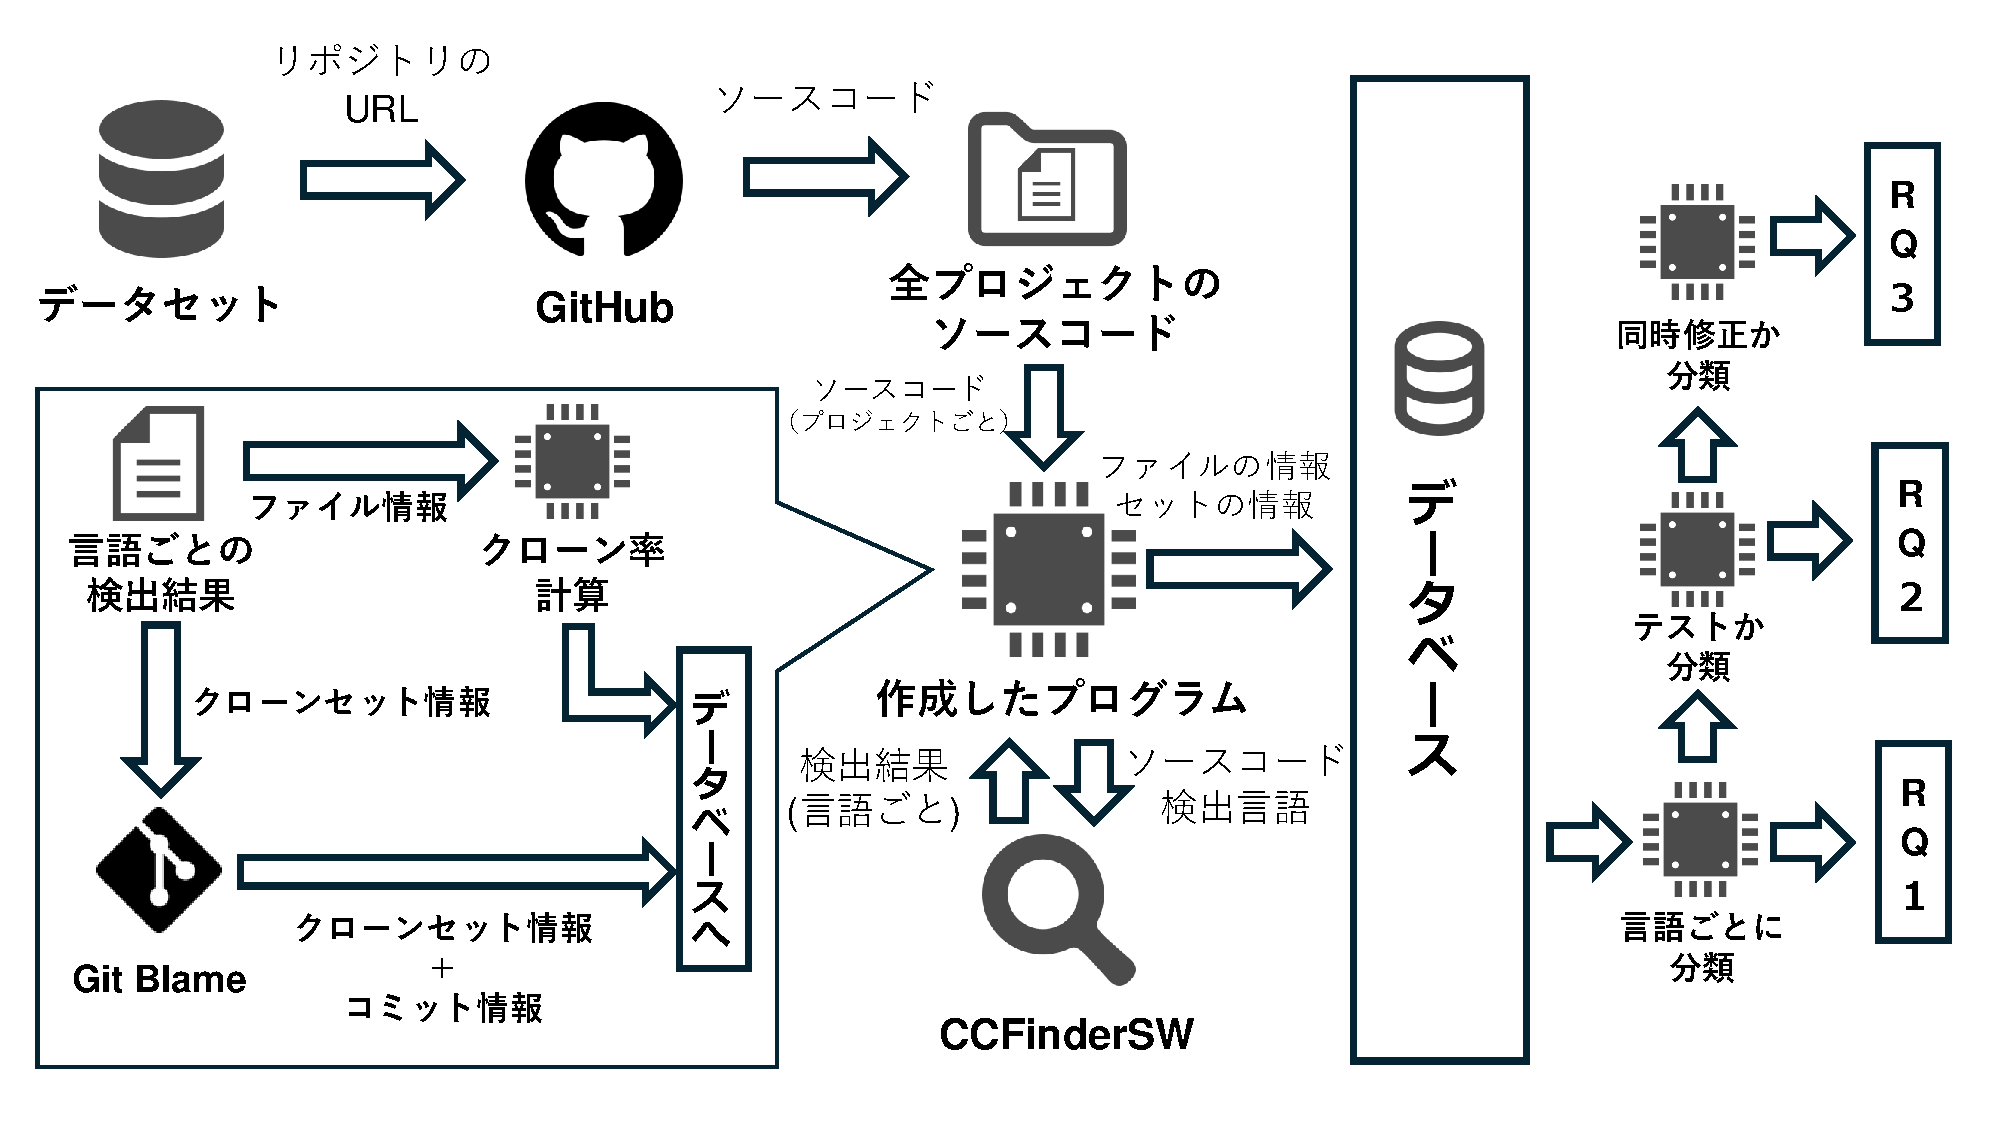
\includegraphics[width=0.8\linewidth]{images/overviewOfMethod.pdf}
    \caption{分析手法の概要}
    \label{fig:overviewOfMethod}
\end{figure*}

%次に,RQに回答するための分析手法の概要を図\ref{fig:overviewOfMethod}に示す.
%これより分析手法について説明する

%図\ref{fig:overviewOfMethod}はRQに回答するための分析手法の概要を示す.
%この図で示すように,最初に2.2節のデータセット\cite{amoroso2024dataset}からGitリポジトリのURLを取得し,GitHubからすべてのプロジェクトのソースコードを\verb|git clone|コマンドで取得する.
%この際,100コミット分のコミットデータも取得する.
%次に,分析手法について説明する.本分析では,\ref{sec:preliminary}章で説明したとおり284個のプロジェクトを分析対象とする.
次に,分析手法について説明する.本分析では,\ref{sec:preliminary}章で説明した284個のプロジェクトを分析対象とする.
図\ref{fig:overviewOfMethod}はRQに回答するために実施する本研究の分析手法の概要を示す.
この図で示すように,d'AragonaらのデータセットからリポジトリのURLを取得し,\verb|git clone|コマンドを用いてGitHubから分析対象のプロジェクトの最新ソースコードを取得する.


%次に取得したソースコードに対して,2.1節で説明したCCFinderSWを用いて,表\ref{table:detectLanguages}にある分析対象の言語それぞれでコードクローンを検出する.
%このとき,予備実験で対象外となったプロジェクトは除外する.
次に,取得したソースコードに対して,CCFinderSWを用いてコードクローンを検出する.
このとき,CCFinderSWの設定は,検出範囲をファイル間に,出力形式をクローンセット,検出するコードクローンの最低トークン数(しきい値)をCCFinderSWのデフォルト値である50トークンに設定した.
検出範囲をファイル間にしたのは,サービス間や機能間のコードクローンを検出するためである.


その後,本分析のために作成したプログラムがCCFinderSWの検出結果ファイルを読み込み,分析に情報を付加してデータベースに格納する.
%これより詳しく説明する.
%まず,CCFinderSWの言語ごとの検出結果が含まれるテキストファイルから,作成したプログラムがファイル情報とクローンセット情報に分ける.
%そのとき,まず,CCFinderSWの言語ごとの検出結果ファイルから,作成したプログラムがファイル情報とクローンセット情報に分ける.
%ファイル情報には,クローン率をファイルごとに算出して付け加える.
このとき,作成したプログラムがCCFinderSWの検出結果ファイルから,ファイル情報とクローンセット情報を取得し,それらの情報をデータベースに格納する.また,ファイルごとのクローン率情報もデータベースに格納する.本研究では,クローン率は$ROC(F)$の値を用いて計算する.
$ROC(F)$はファイル$F$がどの程度重複化しているかを表す指標である.$ROC(F)$は以下の式で計算される.
%Higoらの研究では,ファイル$F$がどの程度重複化しているかを表す指標として,$ROC(F)$を定義している\cite{HIGO2007985}.
%$F$の行数を$LOC(F)$,$F$の$LOC$のうちクローンセットに含まれている$LOC$を$LOC_{duplicated}(F)$とした場合,$ROC(F)$は以下の式で計算される.
\[ROC(F) = \frac{LOC_{duplicated}(F)}{LOC(F)}\]
上の式で,$LOC(F)$は$F$の行数を,$LOC_{duplicated}(F)$は$F$の$LOC$のうちクローンセットに含まれている$LOC$を示す.
これ以降では,$ROC(F)$をクローン率と呼ぶ.
また,クローンセット情報をデータベースに格納するとき,\verb|git blame|コマンドを用いて,クローンセットに含まれているコード片ごとに含まれるコミット情報を付け加える.
%それらの付け加えた情報を含めてクローンセット情報とファイル情報をそれぞれデータベースに格納する.

最後に,データベースに格納された情報を言語ごと,テストコードかプロダクトコードか同時修正されたクローンセットかどうかに基づいて分類し,各RQに回答する.
プロダクトコードとテストコードの区別は以下のとおりである.
\begin{itemize}
    \item ファイルのパス名やファイル名に小文字大文字を区別なく{\sf test}が含まれていたら,そのファイルに含まれるプログラムは全てテストコードとして扱う.
    \item それ以外のファイルは,全てプロダクトコードとして扱う.
\end{itemize}
また,クローンセットがプロダクトコードとテストコードのどちらであるかの判定基準は以下のとおりである.
\begin{itemize}
\item あるクローンセットに含まれるコード片が1つ以上テストコードに含まれていたら,テストコードのクローンセットとする.
\item それ以外(つまり,あるクローンセットに含まれるコード片が全てプロダクトコードに含まれていたら),プロダクトコードのクローンセットとする.
\end{itemize}
以下の手順で,各クローンセットに対して,同時修正が行われたか判定する.この際,最新のコミットから100コミットを分析対象とした.これは,データセット\cite{amoroso2024dataset}に含まれるプロジェクトは,最低100以上のコミットを持つためである.
\begin{description}
    \item[手順1:] クローンセットに含まれる各コード片に対して,クローン検出したバージョンからみて100バージョン以内の修正を列挙し,その中で最も新しい修正を特定する.以上の作業をクローンセットに含まれる全てのコード片に対して行う.
    \item[手順2:] 1.で特定した修正集合の中に,同一コミットが含まれていれば,同時修正が行われたと判定する.さもなくば,同時修正が行われなかったと判定する.
\end{description}


\section{分析結果}

\subsection{RQ1: クローン率が高い言語はどれか?}
%本節の分析では,言語の,4章で説明したクローン率をプロジェクトごとに算出する.
%その後,算出した値を言語間で比較することで分析を行う.
%このRQに応えるため,\ref{sec:analysis}章で定義したクローン率に基づき,プロジェクトごとに各言語の平均クローン率を算出し,算出した値を言語間で比較した.
\ref{sec:analysis}章で定義したクローン率に基づき,プロジェクトごとに各言語の平均クローン率を算出し,算出した値を言語間で比較した.
\begin{figure*}[tb]
    \centering
    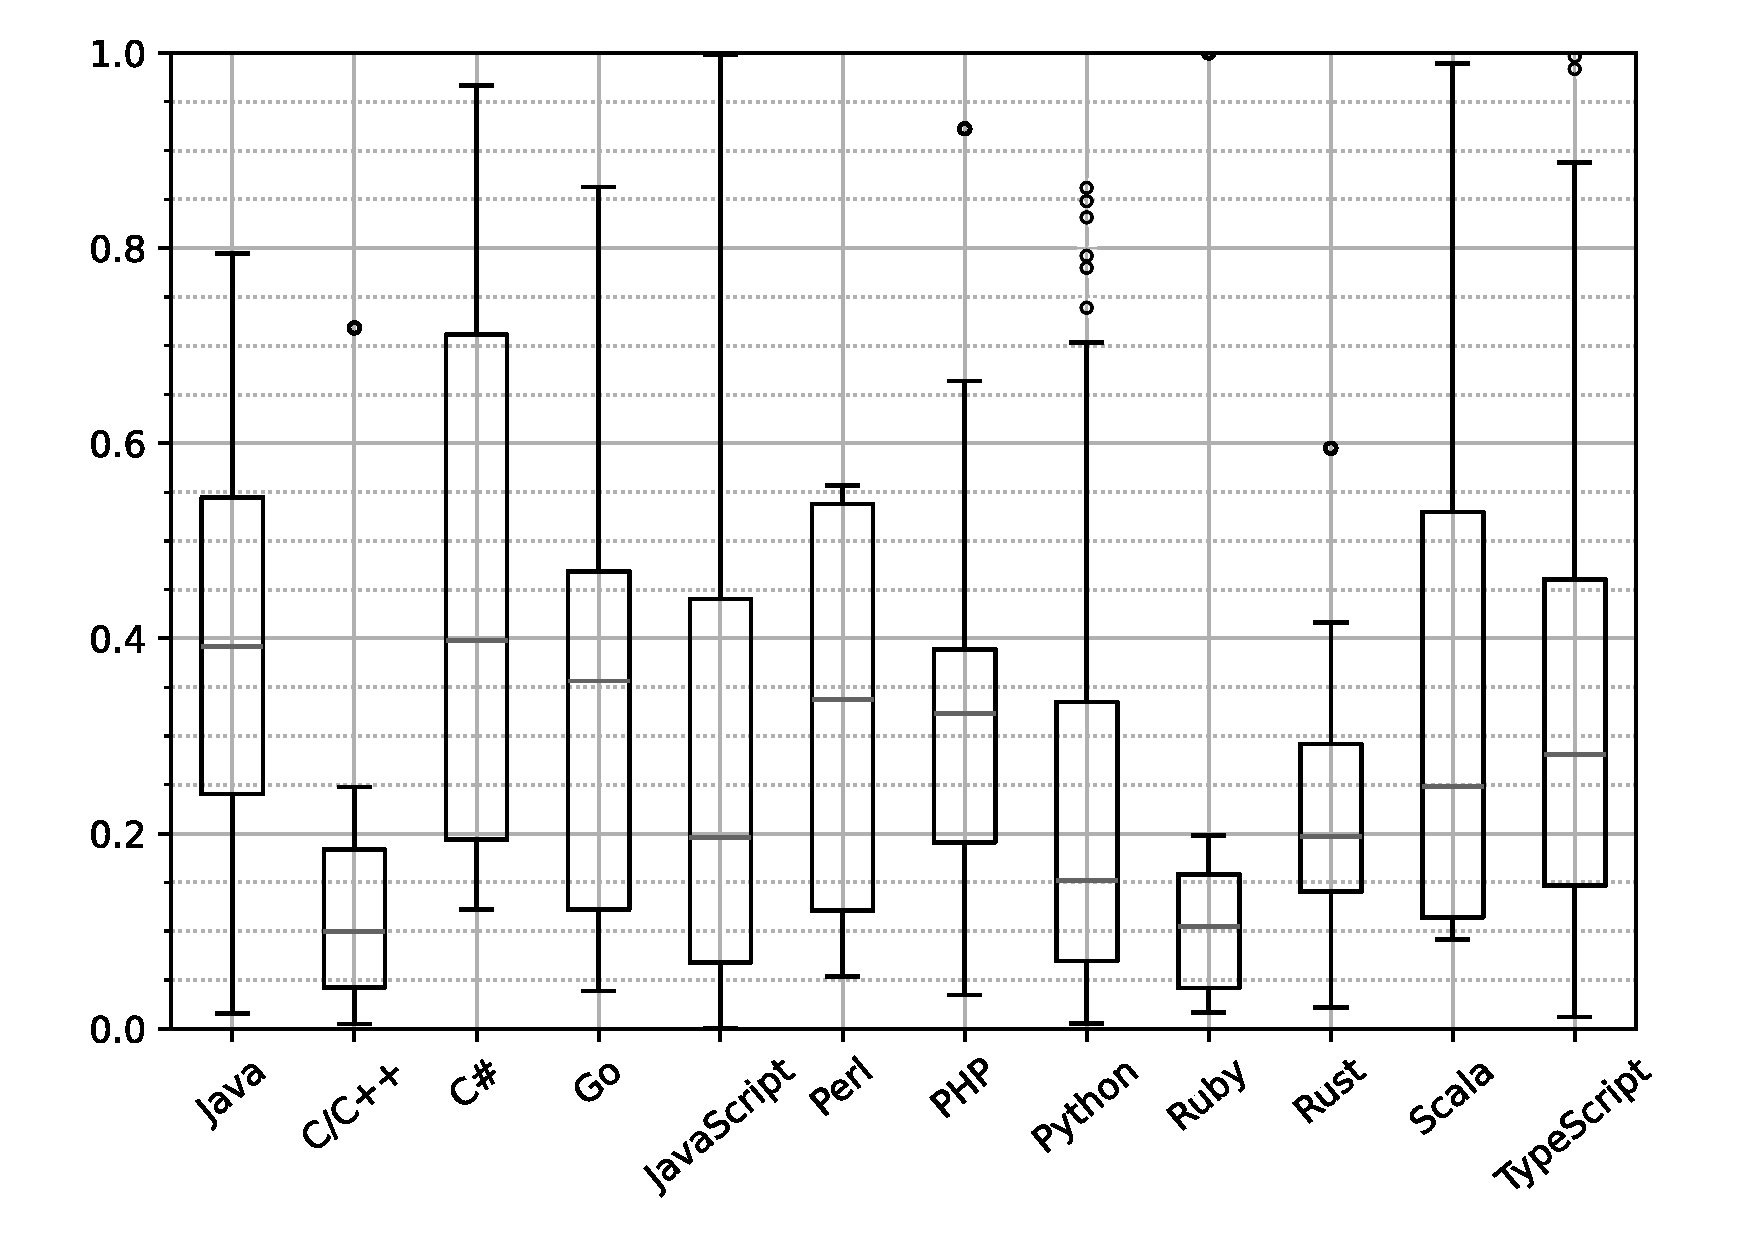
\includegraphics[width=11.0cm]{images/RQ1.pdf}
    \caption{言語ごとのクローン率の箱ひげ図}
    \label{fig:cloneRateByLanguages}
\end{figure*}
%
その分析結果を図\ref{fig:cloneRateByLanguages}に示す.
この図の縦軸はクローン率,横軸は言語を示す.
%また,この図の縦軸はクローン率で,横軸は言語である.

%これより,分析結果を説明する.
図\ref{fig:cloneRateByLanguages}が示すように,
クローン率の中央値が最も高かった言語は,C\#で40\%であった.
C\#に次いで、Javaが39\%、Goが35\%と高い値を示した.
また,最小値に着目すると,C\#は12\%であるのに対し,JavaとGoはそれぞれ1\%と4\%であった.
一方,クローン率の中央値が最も低かった言語は,RubyとC/C++で,いずれも10\%であった.
また,RubyとC/C++は最大値はそれぞれ25\%,20\%であった.

\begin{itembox}[l]{RQ1への回答}
最もクローン率の中央値が高い言語はC\#で40\%であった.
%表現が微妙かも(太田)
2位と3位はJava,Goであり,それぞれ39\%,35\%であった.
%一方,最もクローン率の中央値が低い言語は,C/C++とRubyで10\%であった.
\end{itembox}

%クローンがテストコードである割合はどのくらいか?
\newpage
\subsection{RQ2: プロダクトコードとテストコードでクローン率に違いがあるか?}

%本節では,プロダクトコードとテストコードでクローン率に違いがあるかを分析する.
%この分析は,各言語ごとにプロダクトコードとテストコードのクローン率をプロジェクト単位で算出することで行った.
プロダクトコードとテストコードにおけるクローン率に違いがあるか,言語ごとに分析した.
\begin{figure*}[tb]
    \centering
    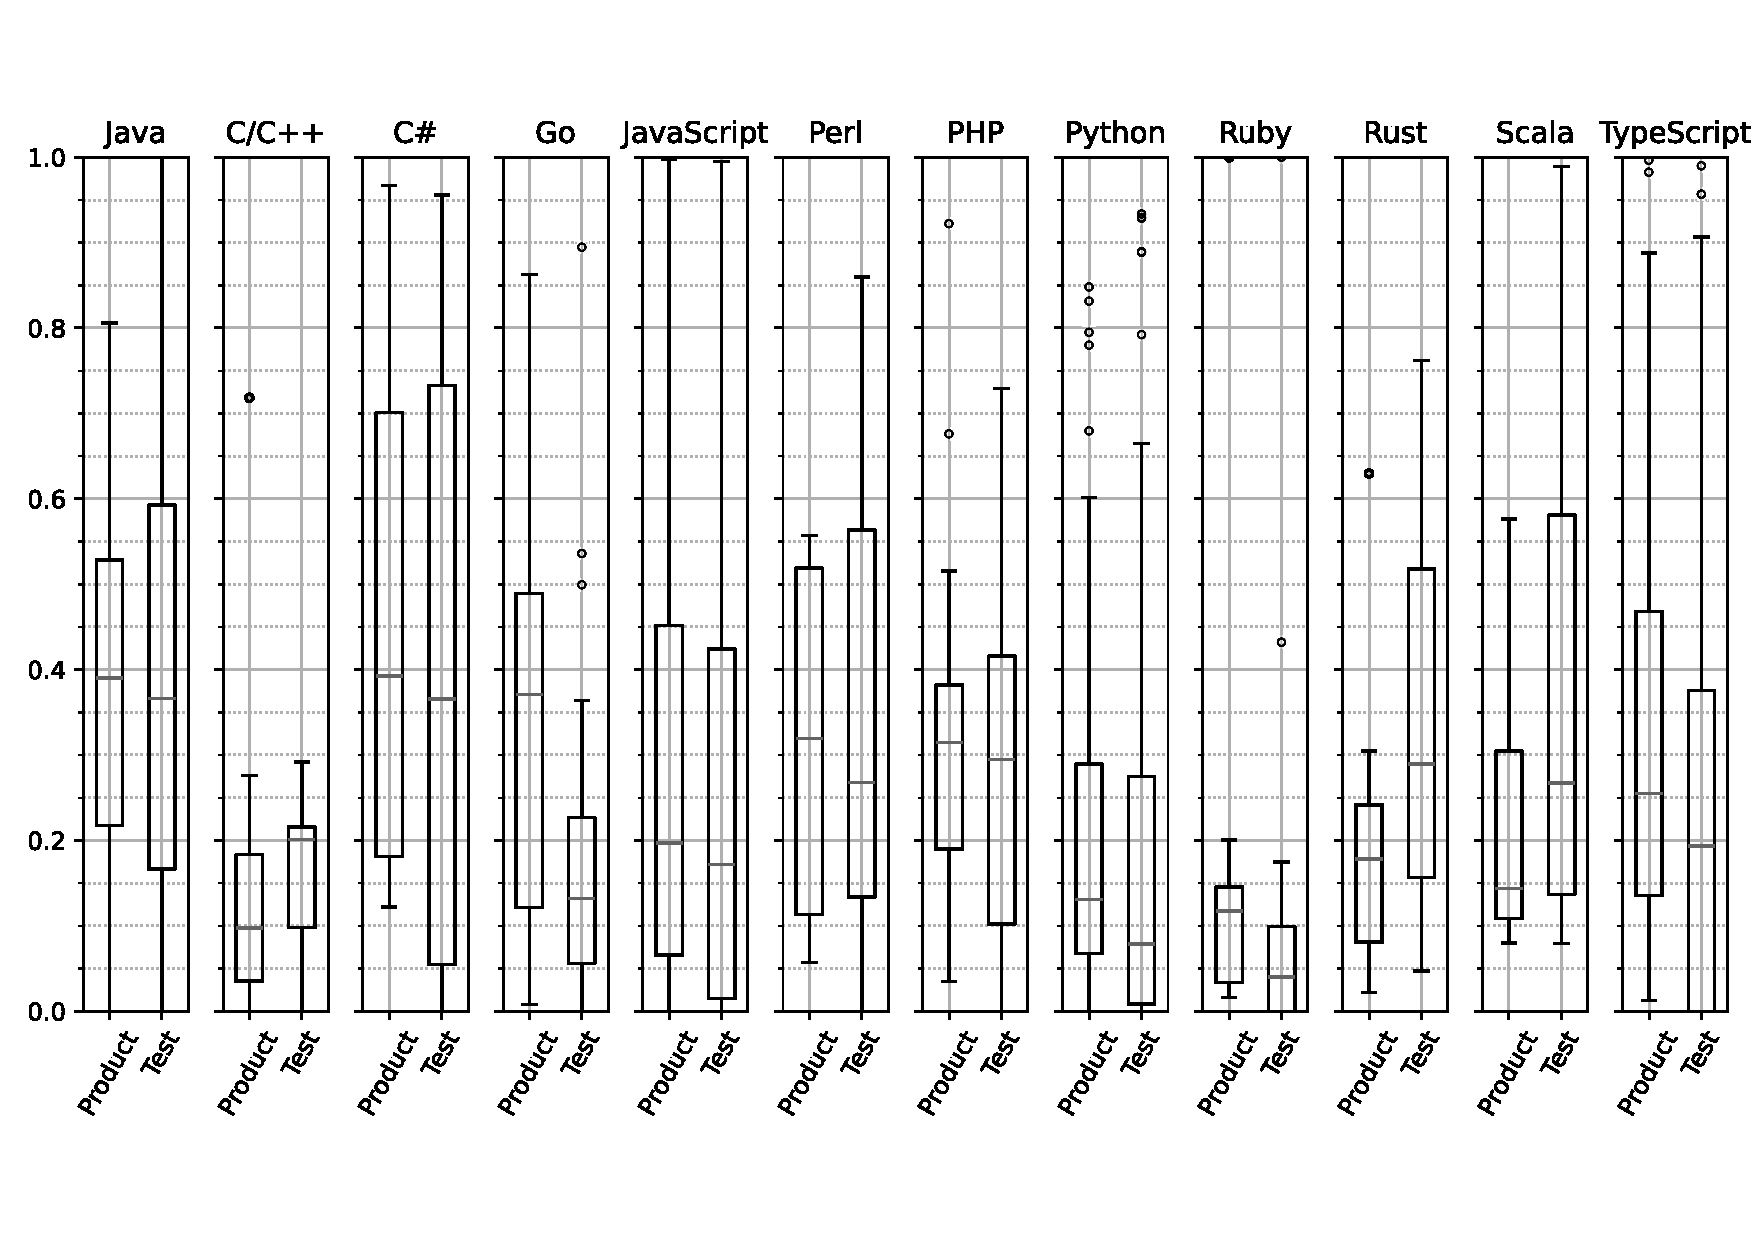
\includegraphics[width=\textwidth]{images/RQ2.pdf}
    \caption{テストコードとプロダクトコードにおける言語ごとのクローン率}
    \label{fig:cloneRateOfTestAndProduct}
\end{figure*}

% \begin{table*}[tb]
%     \centering
%     \caption{言語ごとのプロダクトコードとテストコードのLOCおよびプロジェクト数\\(各プロジェクトが複数言語に該当することがある)}
%     \label{table:numberOfCloneSetCountByLabel}
%     \begin{minipage}{0.495\linewidth}
%     \small
%     \begin{tabular}{|c|r|r|r|r|}
%     \hline
%     言語 & $LOC_p$ & $LOC_t$ & $N_F$ & $N_P$\\
%     \hline \hline
%     Java & 2,745,122 & 1,222,774 & 30,808 &78 \\
%     \hline
%     C/C++ & 398,927 & 57,260 & 2,018 & 13 \\
%     \hline
%     C\# & 564,648 & 15,729 & 8,890 & 20 \\
%     \hline
%     Go & 1,419,113 & 770,226 & 9,888 & 28 \\
%     \hline
%     JavaScript & 7,514,896 & 489,772 & 32457 & 152 \\
%     \hline
%     Perl & 35,085 & 2,677 & 309 & 4 \\
%     \hline \hline
%     全体 & 19,876,981 & 5,121,542 & 1,721,04 & 284 \\
%     \hline \hline
%     \end{tabular}
%     \end{minipage}
%     \begin{minipage}{0.495\linewidth}
%     \small
%     \begin{tabular}{|c|r|r|r|r|}
%     \hline
%     言語 & $LOC_p$ & $LOC_t$ & $N_F$ & $N_P$\\
%     \hline \hline
%     PHP & 1,348,647 & 177,388 & 11,314 & 23 \\
%     \hline
%     Python & 2,298,816 & 1,517,369 & 29,908 & 88 \\
%     \hline
%     Ruby & 690,165 & 108,059 & 12,848 & 14 \\
%     \hline
%     Rust & 527,790 & 253,109 & 4,190 & 10 \\
%     \hline
%     Scala & 301,799 & 214,609 & 4,935 & 10 \\
%     \hline
%     TypeScript & 2,031,973 & 292,570 & 24,539 & 54 \\
%     \hline \hline
%     全体 & 19,876,981 & 5,121,542 & 1,721,04 & 284 \\
%     \hline \hline
%     \end{tabular}
%     \end{minipage}
% \end{table*}
\begin{table}[tb]
    \centering
    \caption{言語ごとのプロダクトコードとテストコードのLOCおよびプロジェクト数\\(各プロジェクトが複数言語に該当することがある)}
    \label{table:numberOfCloneSetCountByLabel}
    \small
    \begin{tabular}{|c|r|r|r|r|}
    \hline
    言語 & K$LOC_p$ & K$LOC_t$ & $N_F$ & $N_P$\\
    \hline \hline
    Java & 2,745 & 1,223 & 30,808 &78 \\
    \hline
    C/C++ & 399 & 57 & 2,018 & 13 \\
    \hline
    C\# & 565 & 16 & 8,890 & 20 \\
    \hline
    Go & 1,419 & 770 & 9,888 & 28 \\
    \hline
    JavaScript & 7,515 & 490 & 32,457 & 152 \\
    \hline
    Perl & 35 & 3 & 309 & 4 \\
    \hline
    PHP & 1,349 & 177 & 11,314 & 23 \\
    \hline
    Python & 2,299 & 1,517 & 29,908 & 88 \\
    \hline
    Ruby & 690 & 108 & 12,848 & 14 \\
    \hline
    Rust & 528 & 253 & 4,190 & 10 \\
    \hline
    Scala & 302 & 215 & 4,935 & 10 \\
    \hline
    TypeScript & 2,032 & 293 & 24,539 & 54 \\
    \hline \hline
    合計 & 19,877 & 5,122 & 1,721,04 & 284 \\
    \hline \hline
    \end{tabular}
\end{table}

テストコードとプロダクトコードの言語ごとのクローン率の分析結果を図\ref{fig:cloneRateOfTestAndProduct} に示す.
この図に示すように,プロダクトコードにおけるクローン率の中央値の上位3言語は,C\#,Java,Goで,それぞれ39\%,39\%,37\%であった.
また,C\#の最小値が12\%である一方,JavaとGoの最小値はそれぞれ0\%と1\%であった.
テストコードでは,クローン率の中央値の上位3言語は,C\#,Java,PHPで,それぞれ37\%,37\%,29\%であった.
また,C\#,Java,PHPのいずれの言語も最小値は0\%であった.
C\#とJavaはプロダクトコードとテストコードの両方で高いクローン率を示した.

また,各言語ごとのプロジェクト数,および言語ごとのプロダクトコードとテストコードの$LOC$を表\ref{table:numberOfCloneSetCountByLabel}に示す.
この表では,$LOC_p$はプロジェクトコードの$LOC$の合計,$LOC_t$はテストコードの$LOC$の合計,$N_F$はファイル数,$N_P$はプロジェクト数を示す.
また,プロジェクト数は1つのプロジェクトに複数の言語が含まれている場合がある.
この表より,いずれの言語でもプロダクトコードとテストコードは十分な量存在することが分かる.

最後に,プロダクトコードとテストコードにおけるクローン率の有意差を,有意水準5\%でマン・ホイットニーのU検定で確かめた.
その結果,GoとPythonでプロダクトコードとテストコードの間に有意な差が見られた.

%これより,図\ref{fig:cloneRateOfTestAndProduct}からわかることを説明する.
%プロダクトコードでは,クローン率の中央値の上位3件は,C\#,Java,Goで,それぞれ39\%,39\%,37\%であった.
%また,テストコードにおける,クローン率の中央値の上位3件は,C\#,Java,PHPで,それぞれ37\%,37\%,29\%であった.

\begin{itembox}[l]{RQ2への回答}
%GoとPythonで,クローン率におけるプロダクトコードとテストコードの有意差が見られた.
%したがって,一部の言語では,プロダクトコードとテストコードのクローン率が異なっているといえる.
GoとPythonで,クローン率におけるプロダクトコードとテストコードの有意差が見られた.
したがって,一部の言語では,プロダクトコードとテストコードのクローン率が異なるといえる.
\end{itembox}


%テストコードで含まれるクローンが修正されやすいか
\subsection{RQ3: コードクローンに対する同時修正率が高い言語はどれか?}
%本節では,コードクローンに対する同時修正率の言語ごとの違いを分析する.
%本分析における同時修正率は,同時修正が発生しているクローンセットの数を全体のクローンセットの数で割ったものである.
%また本節の分析は,テストコードとプロダクトコードを区別して行う.
%このRQに応えるため,コードクローンに対する同時修正率が言語によって異なるか,テストコードとプロダクトコードを区別した分析した.
コードクローンに対する同時修正率が言語によって異なるか,テストコードとプロダクトコードを区別し分析した.
本分析における同時修正率は,同時修正されたクローンセットの数を全体のクローンセットの数で割ったものである.


\begin{figure*}[tb]
    \centering
    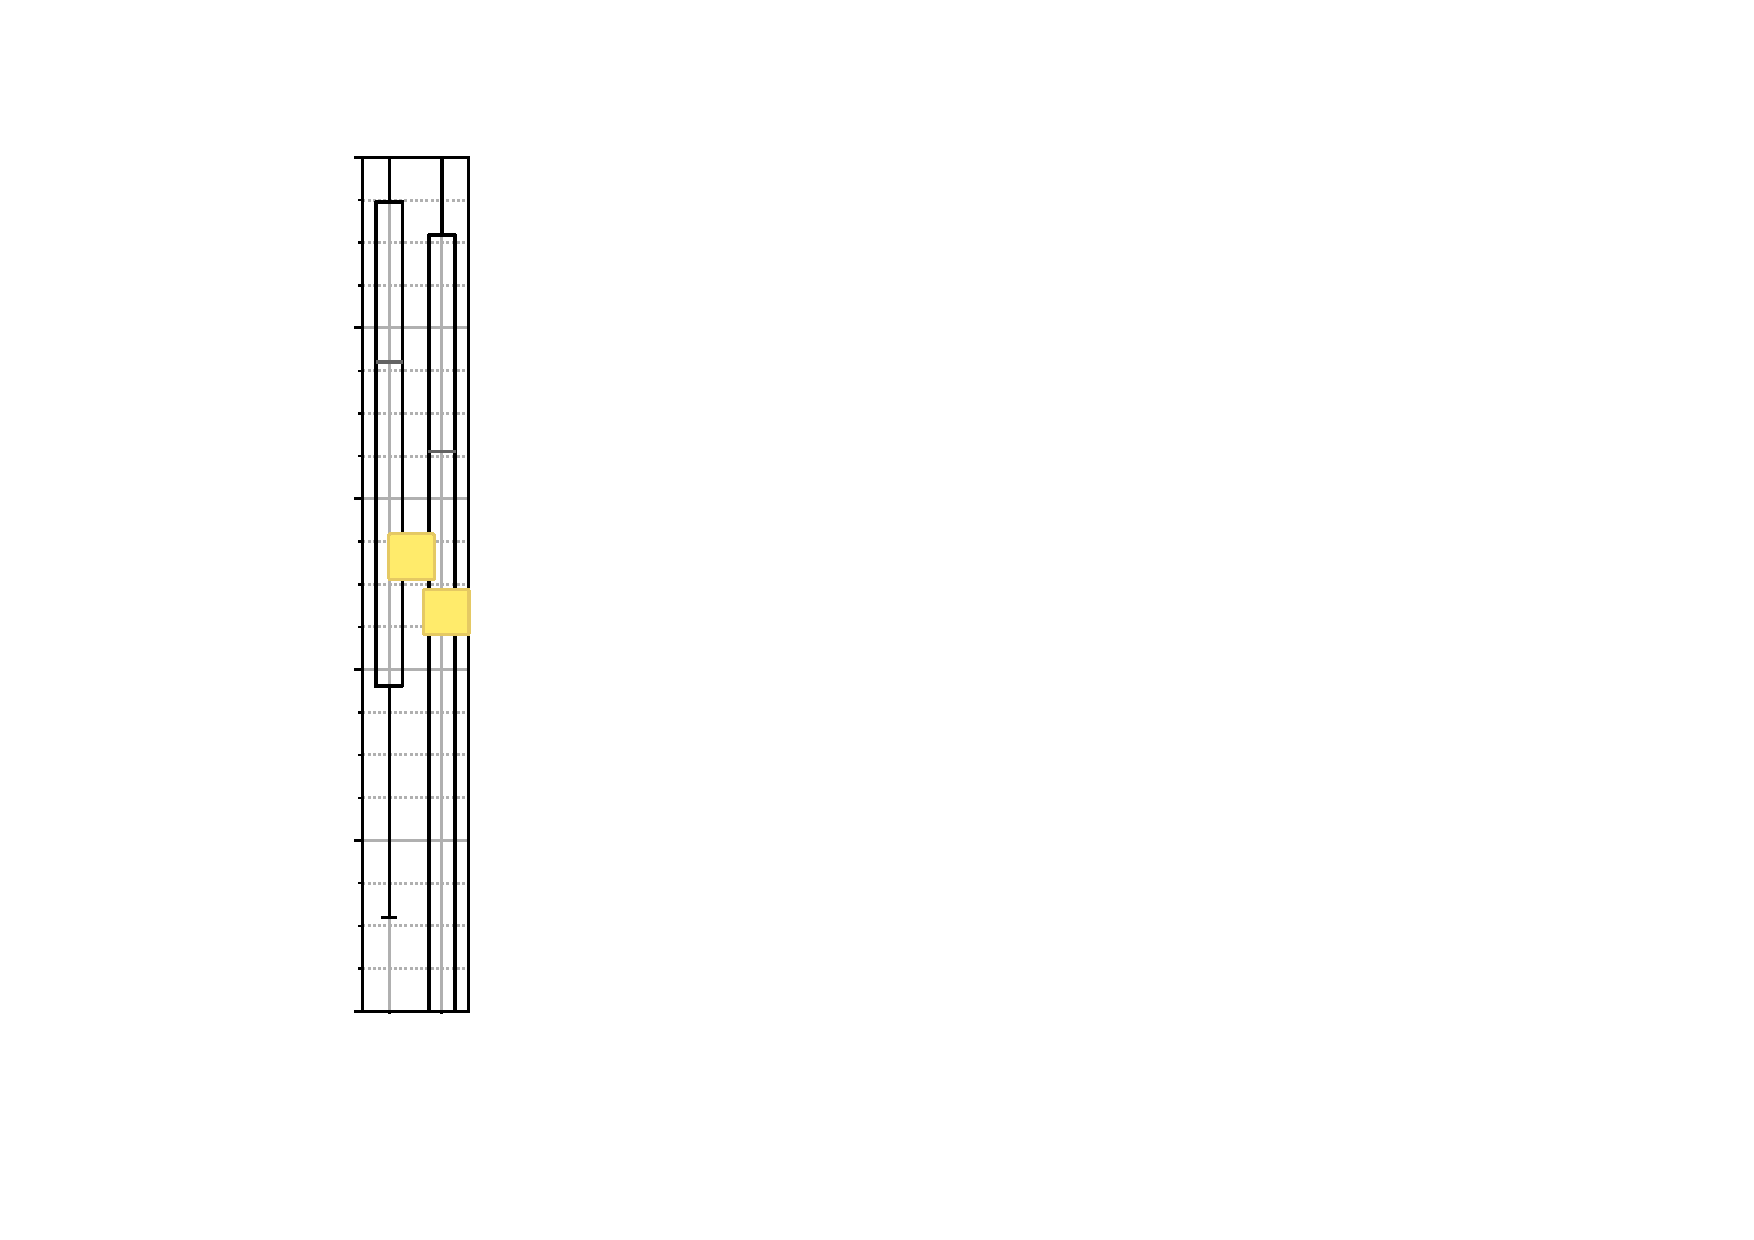
\includegraphics[width=\textwidth]{images/RQ3.pdf}
    \caption{プロダクトコードとテストコードにおける言語ごとの同時修正率}
    \label{fig:rateOfCoModifiedOfTestAndProduct}
\end{figure*}

分析結果を図\ref{fig:rateOfCoModifiedOfTestAndProduct}に示す.
この図では,縦軸にプロジェクトごとの同時修正率を示し,横軸に言語ごとにテストコードとプロダクトコードを分けて示す.
図に示すように,
C\#の同時修正率の中央値が全言語で最も高く,71\%であった.
一方,C/C++とPerlの同時修正率の中央値が全言語で最も低く,1\%であった.
これらの結果から,言語によって同時修正率が異なると明らかになった.
プロダクトコードにおける同時修正率の中央値の上位3件言語はC\#,TypeScript,Javaで,それぞれ76\%,38\%,36\%であった.
これらの言語の最小値に着目すると,C\#は11\%である一方で,TypeScriptとJavaでは0\%であった.
また,テストコードにおける同時修正率の中央値の上位3件言語はC\#,Java,Rubyで,それぞれ66\%,42\%,38\%であった.
これらの言語の最小値は全て0\%であった.

最後に,プロダクトコードとテストコードにおける同時修正率の有意差を,有意水準5\%でマン・ホイットニーのU検定で確かめた.
その結果,TypeScriptで有意な差が見られた.

\begin{itembox}[l]{RQ3への回答}
最も同時修正率の中央値が高かった言語はC\#で,71\%であった.
一方,最も同時修正率の中央値が低かった言語は,C/C++とPerlで,1\%であった.
したがって,言語によって同時修正率が異なるといえる.
また,TypeScriptにおいて,プロダクトコードとテストコードの間で同時修正率に有意差があった.
\end{itembox}

\section{考察}


\subsection{分析結果に対する考察}
%本節では分析結果に対する考察を行う.



%まず,クローン率について,Moらの調査結果\cite{mo2021existence}と本分析の結果を比較する.
%Moらは,サービス内では57.1\%から91.7\%,サービス間では35.7\%から87.5\%がクローンになっていることを報告している.
%しかし,全体のクローンペアに対するType-2クローンペアの割合は,サービス内で11.9\%から27.0\%,サービス間で2.3\%から23.0\%であった.
%一方,本分析では,5.1節の分析結果によると,JavaにおけるType-2のクローン率の中央値は39\%であった.
%このことから,Moらの調査におけるType-2のクローン率よりも,本分析における Javaのクローン率は比較的高い結果であったといえる.

%次に,コードクローンに対する同時修正率について,Moらの調査結果と本分析の結果を比較する.
%はじめに,Moらの研究の調査と本分析では同時修正の定義が異なっていることを断っておく.
%Moらの研究の調査では過去5つのバージョンを比較しているが,本分析では最新のコードのコミット番号を比較している.
%同時修正の定義の違いを踏まえて,これより比較について述べる.
%Moらの調査では,サービス内では同時修正率が28.6\%から60.0\%,サービス間での同時修正率が14.3\%から63.6\%であること報告している.
%しかし,同時修正されたクローンペア全体に対するType-2クローンペアの割合はサービス内で0.0\%から40.0\%,サービス間で0.0\%から50.0\%であると報告されている.
%一方,本分析では,5.3節の分析結果によると,JavaプロダクトコードにおけるType-2クローンセットの同時修正率の中央値は36\%であった.
%このため,Moらの調査におけるType-2の同時修正率よりも,本分析におけるJavaの同時修正率は,比較的高い結果であったといえる.

%続いて,マイクロサービスでないプロジェクトのクローン率の調査と本分析の結果を比較する.
%Goonらの研究では,C/C++のプロジェクトにおけるコメントや空行を省いたクローン率が,おおよそ10\%以下に収まり,高くても18\%であったことが報告されている\cite{7880509}.
%一方,本分析では,5.1節の分析結果より,C/C++のクローン率の中央値は10\%で,最大値は25\%であった.
%ただし,本分析ではコメントや空行を省いておらず,コードクローンの検出範囲もファイル間であるため,クローン率はGoonらの研究結果と比べて高い数値が出ることが考えられる.
%したがって,マイクロサービスではクローン率が高くなる傾向があるといえる.

%次に,テストコードとプロダクトコードの違いについて考察する.
RQ2とRQ2の結果より,プロダクトコードとテストコード間で,クローン率や同時修正率に有意差がある言語が存在した.
RQ2では,GoとPythonにおいて,プロダクトコードとテストコードの間にクローン率に有意な差が見られた.
また,RQ3では,TypeScriptにおいて,プロダクトコードとテストコードの間に同時修正率に有意な差が見られた.
このため,同一言語であってもテストコードかどうかで,コードクローンが保守性に与える影響は異なると考えられる.よって,コードクローンのライブラリ化などの保守支援を検討する際は,プロダクトコードとテストコードを区別する必要があると考えられる.


分析結果より,どの言語のコードクローンが保守性を低下させるかを考察する.
コードクローンの存在はソフトウェアの保守性を低下させる原因の一つとして知られている.
しかし,すべてのコードクローンが保守コストを増大させるわけではない.
コードクローンに変更が発生した際に,変更が伝播することで保守性を低下させる.
既存研究では,プロジェクトの生存期間の間に一度も変更されない,あるいは定常的に変更されないコードクローンが存在することを示している\cite{Yamanaka2013}\cite{Goode2011}.
したがって,クローン率と同時修正率が高い言語が保守性を低下させる.
5.1節より,プロダクトコードでは,クローン率の中央値の上位3言語は,C\#,Java,Goで,それぞれ39\%,39\%,37\%であった.
また,5.3節より,プロダクトコードにおける,同時修正率の中央値の上位3言語はC\#,TypeScript,Javaで,それぞれ76\%,38\%,36\%であった.
これらの結果から,C\#とJavaのクローン率と同時修正率が共に高く,これらの言語のコードクローンが保守性を低下させる.
% これら言語で記述されたサービスは,コードクローンにより保守性が低下していると考えられる.
そのため,コードクローンのライブラリ化などの保守支援が必要であると考えられる.

\subsection{妥当性への脅威}
%本節では分析結果の妥当性への脅威を考察する.

はじめに,コードクローン検出ツールについて考える.
本分析では多様なプログラミング言語に一様に対応するため,クローン検出ツールにCCFinderSWを用いた.
しかし,このツールではType-2までのコードクローンしか検出できない.
したがって,Type-3のコードクローンの分析は本分析では行っていない.

次にクローン検出範囲について考察する.
%Moらの調査では,コードクローンをマイクロサービス内とサービス間に分類して調査を行っていた.
Moらの調査では,コードクローンをマイクロサービス内とサービス間に分類して調査した.
しかし,Moらの調査と比べ,本分析ではデータセットのプロジェクト数が増加したため,クローンセットをサービス間とサービス内のものに手動で分類することが困難であった\cite{mo2021existence}.
したがって,本分析の結果は,サービス内クローンおよびサービス間クローンについて調査した結果ではない.

次に自動生成コードについて考察する.
本分析ではテストコードとプロダクトコードを分けて分析した.
よって,テストコードの関係しているクローンセットによる結果への影響は考慮できている.
しかし,RPCシステムの一種であるgRPC\footnote{\url{https://grpc.io/}}や,オブジェクト指向言語のgetter/setterなどのプロダクトコードに含まれうる自動生成コードが存在する.
通常,自動生成コードの分類は,ソースコードのコメントの分類によって行われる.
今回の分析では,多数の言語の分析を行うため,その言語ごとに異なった手法で分類を行う必要がある.
したがって,本分析の結果には自動生成コードによる結果への影響は考えられていない.

次にテストコードの定義について考察する.
本分析では,クローンセットに1つでもテストコードが含まれていれば,テストコードのクローンセットとして扱った.しかし,プロダクトコードとテストコードを分けてクローン検出を行う手法も存在する.したがって,その場合の結果は本分析では考えられていない.

次に言語ごとの特徴について考察する.
本分析ではクローンの検出範囲をファイル間に限定している.
しかし,Javaであれば1ファイルに1クラス,Pythonであれば1ファイルに1モジュールなど,言語ごとに1ファイルに含まれうる単位が異なる.
したがって,言語ごとのファイル構造の違いに起因する結果の変動は考慮できていない.
また,プロジェクト内での用いられ方が言語ごとに異なる場合がある.
さらに,言語ごとに用いられるフレームワークが異なっている.
しかし,本分析ではコードクローンの発生要因の分析は行なっていない.
したがって,言語ごとの用いられ方やフレームワークによる結果への影響は考慮できていない.

最後に,同時修正の定義について考察する.
本分析では同時修正の判定をコミット番号で行っている.
しかし,コミット自体を複数に分けた上で単一マージで取り込んで整合性を取る場合は同時修正と判定できていない.
また,本分析では先行研究\cite{mo2021existence}とは異なり,最新版のクローンのみを同時修正の判定に用いている.
これは,大規模なデータセットに対応するためである.
したがって,本分析の結果はこれらによる影響は考えられていない.


\section{まとめ}
本稿では,Moらの調査結果を踏まえて,多言語かつ大規模なOSSのマイクロサービスのデータセットに対するコードクローンの分析を行った\cite{mo2021existence}.
予備調査ではデータセットのプロジェクトにどのような言語が含まれるかを調査した.
分析はプロジェクト数が多いデータセットに対して処理を行い,RQごとに言語,テスト,同時修正の有無で分類することで行った.
その分析結果は,マイクロサービスでは言語ごと,テストコードとプロダクトコードでコードクローンが異なった性質を持つことを示した.
また,JavaとC\#のコードクローンが他の言語と比べ保守性を低下させることも示した.

今後の展望として,以下が挙げられる.
\begin{itemize}
    \item%[Type-3クローンの分析:] 
    Moらの調査ではType-3クローンを検出し調査を行っていた.しかし,本分析では,対象とする言語を増やしたことによって,それに対応できるType-3クローン検出ツールが存在しなかった\footnote{多様な言語に対応可能なType-3クローン検出ツールとしてMSCCD\cite{MSCCD}が挙げられるが,本分析で対象としたPerlに非対応であり,ScalaやRubyのプログラムに対してコンパイルエラーが発生することある.}.したがって,そのようなコードクローン検出ツールが開発された際の課題とする.
    \item%[サービス内とサービス間への分類:] 
    マイクロサービスでは,サービス間のコードクローンが独立性を脅かす.Moらの調査ではクローンペアをサービス内とサービス間に分類していた.しかし,本分析ではデータセットの規模が大きくなったことで分類が困難になり,行えなかった. そこで,大規模なデータセットにも対応可能な分類手法を今後考案する.
    \item%[自動生成コードの分類:] 
    自動生成コードがプロダクトコードのコードクローンの結果に影響を与えていることが考えられる.しかし,本分析では自動生成コードを分類した分析が行えていない.したがって,多言語なデータセットにも対応可能な自動生成コードの分類手法を今後考案する必要がある.
    \item%[テストコードを分けたクローン検出:]
    本分析は,プロダクトコードとテストコードを分けてクローン検出を行っていない.したがって,プロダクトコードとテストコードを分けてクローン検出を行った結果の分析を今後行う.
    \item%[言語による違いの原因の調査:]
    本分析の考察ではC\#とJavaのコードクローンが他の言語よりも保守性を低下させると結論付けた.しかし,この言語による結果の違いが何に起因するかは分かっていない.したがって,言語による結果の違いの原因を今後調査する.
\end{itemize}

\textbf{謝辞}\
本研究は,JST さきがけ JPMJPR21PAならびにJSPS科研費 JP24K02923,JP20K11745,JP23K11046の支援を受けた.

\bibliographystyle{jssst}
\bibliography{ref}

\end{document}